\chapter{Implementation}
\label{ch:impl}

In this chapter a prototype implementation of the concept introduced in Chapter
\ref{ch:concept} is presented. The chapter is divided in three sections. By
showing a few usage examples, the first part gives an impression on how the
implemented \ac{KVS} can be used. The second part deals with the architecture of
Midas and outlines selected topics such as NVRAM handling and the components
involved in transaction management. The last section delves into the details of
transaction processing and the underlying algorithms. In order to make
addressing the \ac{KVS} more convenient, it is henceforth referred to by its
working title \emph{Midas} \footnotemark.

\footnotetext{The name is taken from Greek mythology. According to the legend,
King Midas was given the ability to turn everything he touches into gold. This
resembles the idea of making information non-volatile as in \ac{NVRAM}.}

\section{Usage Examples}
\label{ch:impl-usage}
In order to get an understanding of how Midas can be used, this section presents
a selected set of usage examples. The first example deals with how an instance
of Midas is created or recovered, respectively. The remaining examples showcase
the transaction API of Midas.

Before Midas can be instantiated, an underlying persistent object pool must be
created or recovered from the file system. Details on object pools are given in
the next section. Once the object pool is initialized, Midas can be instantiated
and transactions can be performed. The example is given in
Listing~\ref{lst:usage-init}.

\begin{lstlisting}[caption={Midas Bootstrapping.},captionpos=b, label=lst:usage-init]
#include "midas.hpp"

/* declarations for this example */

int main() {
    // Create persistent object pool
    midas::pop_type pop;

    // Initial size of the object pool (here: 1GB)
    const size_t pop_size = 1024ULL * 1024 * 1024;

    // Initialize persistent object pool from file.
    if (!midas::init(pop, "midas.db", pop_size))
        return EXIT_FAILURE;

    // Create Midas key-value store based on object pool
    midas::Store store(pop);

    // Run example transactions
    run_single_transaction(store);
    run_concurrent_transactions(store);

    return EXIT_SUCCESS;
}
\end{lstlisting}

Midas uses an ordinary transaction API. In order to execute a transaction, it
must first be started with a call to \code{Store::begin()} which yields a handle
to the new transaction. Using the transaction handle, the store can be modified
in the context of the associated transaction. The available modifiers are
\code{Store::put()}, \code{Store::get()}, and \code{Store::drop()}. As a
compromise between usability and flexibility, the store supports strings as keys
and values, exclusively. Unless a transaction is aborted prematurely, it must
be concluded with a call to \code{Store::commit()}.

\begin{lstlisting}[caption={A single transaction on account data.},captionpos=b, label=lst:usage-single-tx]
void run_single_transaction(midas::Store& store) {
    midas::Transaction::ptr tx = store.begin();

    std::string deb = store.get("debit", tx);
    std::string sav = store.get("saving", tx);
    if (get_balance(sav, deb) < 0.0)
        store.put("debit", apply_interest(deb), tx);

    if (!store->commit(tx))
        // Error: transaction failed
}
\end{lstlisting}

The resulting return code denotes whether the transaction committed successfully
or failed. The following example shows a transaction checking the balance of an
account and applying an interest fee if the balance is negative (see
Listing~\ref{lst:usage-single-tx}).

Running transactions in concurrent threads requires no additional setup other
than creating the respective threads to begin with. Each thread only needs a
reference to the Midas store. While the store is a global resource, each
transaction buffers its updates in its private memory region. The last example
starts 10 threads which all execute the accounting transaction from
Listing~\ref{lst:usage-single-tx}. Because this transaction may modify a value
that is read by all concurrent transactions, many transactions are bound to fail
due to read-write conflicts. The example is shown in
Listing~\ref{lst:usage-concurrent-tx}.

\vspace{0.5cm}

\begin{lstlisting}[caption={Several concurrent accounting transactions on the same store.},captionpos=b, label=lst:usage-concurrent-tx]
void run_concurrent_transactions(midas::Store& store) {
    std::vector<std::thread> threads;
    for (unsigned i=0; i<10; ++i)
        threads.push_back(
            std::thread([&](){ run_single_transaction(store); }));

    for (auto& t : threads)
        t.join();
}
\end{lstlisting}


\clearpage

\section{Architecture}
\label{ch:impl-arch}
\todo[inline]{impl: describe architecture of the store (layers, components)}

\subsection{NVRAM Management}
\label{ch:impl-pmdk}

As explained in Chapter \ref{ch:nvram} there are several challenges to the integration of NVRAM into current systems.

\begin{itemize}
    \item Accessing NVRAM
    \item Programming against NVRAM
    \begin{itemize}
        \item Separation of volatile from non-volatile data
        \item Recovery of non-volatile objects after restart
        \item Ensuring consistency across restarts
    \end{itemize}
\end{itemize}

PMDK (formerly known as NVML) addresses all these problems.

\subsubsection{NVRAM Access}

In PMDK, NVRAM is accessed via ordinary filesystems such as \code{ext4} or \code{tmpfs}. That way, NVRAM can be mapped into a process' address space via plain files. Using a novel kernel feature called \code{DAX} (for direct access) programs can bypass the operating systems page cache. As a result, true load and store semantics are feasible. Ideally, swapping is disabled for the respective memory region.

\subsubsection{Programming Model}

A persistent object pool holds all data that are meant to be durable. Memory inside the object pool is managed by a designated memory allocator. For each object which is meant to be durable, it allocates the required amount of memory and registers the resulting object in the object pool. This way, all objects can be recovered on restart.

In order to separate volatile from non-volatile objects, there are templated wrapper classes to manage integral values and dynamically allocated objects:

\begin{itemize}
    \item \code{pmdk::p<T>} for durable integral values
    \item \code{pmdk::persistent\_ptr<T>} for pointers to durable objects
\end{itemize}

A \code{persistent\_ptr} consists of a non-volatile unique object id and a virtual memory address within the object pool. The virtual address is volatile because it is not valid across restarts. Therefore, the object id is mapped to a relative memory address within the object pool. Using the object id, the virtual memory address of an object can be computed from its relative address to the pool base on every restart.

\todo[inline]{consistency: transactions, trivially-default-constructible classes (objects are only nulled)}
\todo[inline]{consistency: flushing custom or based on transaction state}
\todo[inline]{consistency: ADR}

% =============================================================================
% =============================================================================
% =============================================================================

\subsection{Durable Data Structures}
\label{ch:impl-data}

\subsubsection{Linked List}

\subsubsection{Hash Table}

% * policy-based design for
%     * hashing volatile and non-volatile keys
%         * user does not know about a different represent. of obj. in pmem
%         * volatile keys must have equal hashes with non-volatile counterparts
%         * for safety many hash functions are not equal across restarts
%             * => cannot find pairs after restart
%             * => a) use fixed hash function (impl. from JDK)
%             * => b) rehash entire table (expensive!)
%     * memory management (initial size, load factor, growth factor)
% * conflict handling
%     * chaining (pairs of colliding keys are inserted in a list (aka bucket))
%     * use linked list for buckets
%     * => table is array of buckets

% =============================================================================
% =============================================================================
% =============================================================================

\subsection{Serializable MVCC}
\label{ch:impl-mvcc}

\subsubsection{Transactions}

\subsubsection{Versioning}
\paragraph{Versions}
\paragraph{Histories}
\paragraph{Visibility}

\subsubsection{Conflicts}


\section{Transaction Processing}
\label{ch:impl-tx}
Unlike other \acp{KVS}, Midas can only be operated through transactions. Transactions that are either terminated or belong to another store instance are rejected. Once a transaction has been started with \code{Store::begin()}, it can be used to access the store with \code{Store::read()}, \code{Store::write()}, and \code{Store::drop()}. For the full list of procedures, see Table \ref{tab:procedures}.

% \begin{itemize}
%     \item read: \code{Store::read(<tx>, <key>, <value>)}
%     \item update: \code{Store::write(<tx>, <key>, <value>)}
%     \item deletion: \code{Store::drop(<tx>, <key>)}
% \end{itemize}

% \begin{figure}[!ht]
%     \centering
%     \begin{tabular}{|l|l|}
%         \hline
%         \textbf{Operation} & \textbf{Procedure} \\
%         \hline
%         \hline
%         Begin  & \code{begin() : tx\_ptr} \\
%         Abort  & \code{abort(tx\_ptr) : int} \\
%         Commit & \code{commit(tx\_ptr) : int} \\
%         Read   & \code{read(tx\_ptr, const key\_type\&, value\_type\&) : int} \\
%         Update & \code{write(tx\_ptr, const key\_type\&, value\_type\&) : int} \\
%         Delete & \code{drop(tx\_ptr, const key\_type\&) : int} \\
%         \hline
%     \end{tabular}
%     \caption{An overview of all procedures provided by Midas.}
%     \label{tab:procedures}
% \end{figure}

% \begin{figure}[!ht]
\begin{table}[!ht]
    \centering
    \begin{tabular}{|l|ll|}
        \hline
        \textbf{Operation} & \textbf{Procedure} & \\
        \hline
        \hline
        Begin  & \code{begin()} & \code{: tx\_ptr} \\
        Abort  & \code{abort(tx\_ptr)} & \code{: int} \\
        Commit & \code{commit(tx\_ptr)} & \code{: int} \\
        \hline
        Read   & \code{read(tx\_ptr, const key\_type\&, value\_type\&)} & \code{: int} \\
        Update & \code{write(tx\_ptr, const key\_type\&, value\_type\&)} & \code{: int} \\
        Delete & \code{drop(tx\_ptr, const key\_type\&)} & \code{: int} \\
        \hline
    \end{tabular}
    \caption{An overview of all procedures provided by Midas.}
    \label{tab:procedures}
% \end{figure}
\end{table}

%\begin{lstlisting}
%class Store {
%public:
%    tx_ptr begin();
%    int abort(tx_ptr tx, int reason);
%    int commit(tx_ptr tx);
%    int read(tx_ptr tx, const key_type& key, mapped_type& result);
%    int write(tx_ptr tx, const key_type& key, const mapped_type& value);
%    int drop(tx_ptr tx, const key_type& key);
%
%    // ...
%};
%\end{lstlisting}

Each operation has its own procedure. The control flow of most procedures is structured in the same way. At first, inputs are checked for errors. Next, the history of the item associated with the specified key is looked up. While \code{Store::read()} and \code{Store::drop()} will fail if no history is found, \code{Store::write()} will perform an insertion by adding a new pair to the transaction's change set. If a history is found, then it is scanned for a version that is visible to the specified transaction. If a valid version is found, the operation can perform its read, write, or deletion, respectively. Otherwise, the operation cannot continue and aborts the associated transaction with an error code. Finally, a transaction must be committed with \code{store::commit()} to make its changes durable. Until then, it can always be aborted with \code{Store::abort()}. The subsequent sections give details about the implementations of visibility, operations, and commits.

\subsection{Visibility}
\label{ch:impl-vsb}

A transaction can only access an item if that item's history contains a version that is visible to the transaction. Therefore, transactions have to scan the histories of all items that they wish to access. During the linear search on a history, for each version, a visibility test is performed. There is at most one version visible to a transaction, if any.

Since Midas is based on SI, it features the same visibility conditions. Simply
put, a version $v_0$ is visible to a transaction $t_1$, when $v_0$ was committed
before $t_1$ started. There are several facets to this property. For instance,
during $t_1$'s runtime, another transaction $t_2$ may have updated $v_0$ but has
not yet committed. In this case, $t_1$ can still see $v_0$ because, $t_2$ may
still fail or get aborted. For this to work, $t_1$ must be able to see that
$v_0$ was touched by $t_2$. Therefore, when a transaction $t$ updates or deletes
a version $v$, $t$ replaces $v$'s end timestamp with the TID of $t$. This way,
$t_1$ can see that $v_0$ was updated, lookup $t_2$ in the transaction table, and
inspect its current status. Likewise, if $t_2$ encounters a version $v_1$ that
was created by $t_1$, then $t_2$ would find $t_1$'s TID in the begin timestamp
field of $v_1$. When a transaction commits, it changes its status to
\code{Committed} and propagates its own end timestamp to all versions it has
created or modified. But other transactions do not have to wait until the
propagation is finished, because, using the deposited TID, they can always
lookup the respective transaction and see that its status has changed to
\code{Committed}.

\begin{algorithm}
\begin{algorithmic}[1]
\Procedure{isVisible}{tx, begin, end}
\If {$\text{isTID}(\textit{begin})$}
\State $\textit{tx}^{*} \gets \text{getTx}(\textit{begin})$
% \If {$\text{getStatus}(\textit{tx}^{*}) \neq \text{Committed} \lor \text{getEnd}(\textit{tx}^{*}) > \text{getBegin}(\textit{tx})$}
\If {$\text{getStatus}(\textit{tx}^{*}) \neq \text{Committed} \textbf{ or } \text{getEnd}(\textit{tx}^{*}) > \text{getBegin}(\textit{tx})$}
\State \Return $\text{false}$
\EndIf
\Else
\If {$\textit{begin} >= \text{getBegin}(tx)$}
\State \Return $\text{false}$
\EndIf
\EndIf
\State
\If {$\text{isTID}(\textit{end})$}
\State $\textit{tx}^{*} \gets \text{getTx}(\textit{end})$
% \If {$\text{getStatus}(\textit{tx}^{*}) = \text{Committed} \land \text{getEnd}(\textit{tx}^{*}) < \text{getBegin}(\textit{tx})$}
\If {$\text{getStatus}(\textit{tx}^{*}) = \text{Committed} \textbf{ and } \text{getEnd}(\textit{tx}^{*}) < \text{getBegin}(\textit{tx})$}
\State \Return $\text{false}$
\EndIf
\Else
\If {$\textit{end} < \text{getBegin}(tx)$}
\State \Return $\text{false}$
\EndIf
\EndIf
\State \Return $\text{true}$
\EndProcedure
\end{algorithmic}
\caption{}
\label{alg:vsb}
\end{algorithm}

Visibility test of a single version first inspects its begin timestamp and then its end timestamp. As explained earlier, the value domains of TIDs and timestamps are disjoint in that the former are always odd while the latter are even. Therefore, it is sufficient for a transaction to test the least significant bit of the timestamp to distinguish TIDs from timestamps. A pseudo code example of the visibility test in Midas is outlined in Algorithm \ref{alg:vsb}. The visibility properties implemented in Midas are based on
the works of \cite{berenson1995critique, larson2011high}.

% \vspace{0.5cm}

% \vfill

\subsection{Reads}

The read operation is the simplest operation to perform with Midas. Still, with regard to serializability, reads are very important, because this is where Midas extends SI. Reads are performed by calling \code{Store::read()} and are implemented as follows. A pseudo code example is given below (see Algorithm \ref{alg:read}). After initial input sanitization, it is checked whether the specified item has already been updated within the same transaction. In this case, the item's updated value is retrieved from the change set and the operation returns. Otherwise, the history associated with the given key is looked up. Note that the index is locked for the duration of the lookup. If no history is found, the current transaction is aborted.

\begin{algorithm}[!ht]
\begin{algorithmic}[1]
\Procedure{read}{tx, key, value}
\If {$\text{inChangeSet}(\textit{tx, key})$}
\State $\textit{value} \gets \text{getChangeEntry}(tx, key)$
\State \Return $\text{OK}$
\EndIf
\State $\textit{history} \gets \text{getHistory}(\textit{key})$
\If {$!\textit{history}$}
\State \Return $\text{abort}(tx)$
\EndIf
\State $\textit{snapshot} \gets \text{getReadSnapshot}(\textit{tx, history})$
\If {$!\textit{snapshot}$}
\State \Return $\text{abort}(tx)$
\EndIf
\State $\text{updateReadSet}(\textit{tx, snapshot})$
\State $\textit{value} \gets \text{getData}(snapshot)$
\State \Return $\text{OK}$
\EndProcedure
\end{algorithmic}
\caption{}
\label{alg:read}
\end{algorithm}

From the history, a readable version (i.e. \emph{snapshot}) of the target item is determined. The call to \code{getReadSnapshot()} is where the visibility test from Section \ref{ch:impl-vsb} comes into action. If this fails, the transaction has to abort. Note that for the duration of \code{getReadSnapshot()}, the respective history is locked. When a valid snapshot is found, it is registered in the read set of the transaction. This is necessary to detect potential read-write conflicts at the end of the transaction and thus enable serializability. After the read set has been updated, the snapshots payload can be retrieved and written to the output parameter \code{value}.

\subsection{Updates}

The update operation in Midas is called \code{Store::write()}. It can be used to update existing items and insert new items. Because there can be no duplicates, Midas can always determine which action to perform. A pseudo code of the implementation is given in Algorithm \ref{alg:update}. As before, it is first checked whether the specified item has already been modified in the context of the current transaction \code{tx}. If so, the change set is updated with the new value. In case the change entry indicates that the item was previously removed by \code{tx}, the operation descriptor is changed from \code{mode::remove} to \code{mode::update}. This is possible because, due to the two-level store architecture, all updates and deletions are buffered until commit. If the target item is not in the change set, Midas proceeds as usual and looks up the item's version history.

\begin{algorithm}
\begin{algorithmic}[1]
\Procedure{write}{tx, key, value}
\If {$\text{inChangeSet}(\textit{tx, key})$}
\State $\text{updateChangeSet}(tx, key, value)$
\State \Return $\text{OK}$
\EndIf
\State $\textit{history} \gets \text{getHistory}(\textit{key})$
\If {$!\textit{history}$}
\State \Return $\text{insert}(\textit{tx, key, value})$
\EndIf
\State $\textit{snapshot} \gets \text{getWriteSnapshot}(\textit{tx, history})$
\If {$!\textit{snapshot}$}
\State \Return $\text{abort}(tx)$
\EndIf
\State $\text{setEndTS}(snapshot, \text{getId}(tx))$
\State $\text{updateChangeSet}(\textit{tx, mode::update, snapshot, value})$
\State \Return $\text{OK}$
\EndProcedure
\end{algorithmic}
\caption{}
\label{alg:update}
\end{algorithm}

Unlike with reads, a missing history is not a reason to abort but indicates that a new version must be inserted. If a history exists, then a writable snapshot is determined. Note that there is no insertion if \code{getWriteSnapshot()} fails, because that indicates a write-write conflict. In this case, the most suitable version must have been invalidated with the TID of a transaction other than the current \code{tx}. Therefore, \code{tx} must abort according to the \emph{first-updater-wins} principle seen in Section \ref{ch:kvs-cc-conflicts}. If a valid snapshot is found, its end timestamp is atomically replaced with the TID of \code{tx}. Finally, a new change set entry is created and the operation is complete. Note that, apart from replacing the snapshots timestamp, no NVRAM is updated at this point.

\subsection{Deletions}

An item can be deleted by invoking \code{Store::drop()}. Deletion is very similar to updating. The corresponding pseudo code is shown in Algorithm \ref{alg:delete}. As with updates, the change set is first checked for an existing change entry. If an entry exists, then there are two possibilities: the entry denotes an insertion and is is deleted immediately or it denotes an update in which case the operation descriptor is changed from \code{mode::update} to \code{mode::remove}. In contrast to updating, deletion must abort if no history is found for the specified key. The rest of the function works like \code{Store::write()} (see Algorithm \ref{alg:update}).

\begin{algorithm}
\begin{algorithmic}[1]
\Procedure{drop}{tx, key}
\If {$\text{inChangeSet}(\textit{tx, key})$}
\State $\text{updateChangeSet}(tx, key, value)$
\State \Return $\text{OK}$
\EndIf
\State $\textit{history} \gets \text{getHistory}(\textit{key})$
\If {$!\textit{history}$}
\State \Return $\text{abort}(tx)$
\EndIf
\State $\textit{snapshot} \gets \text{getWriteSnapshot}(\textit{tx, history})$
\If {$!\textit{snapshot}$}
\State \Return $\text{abort}(\textit{tx})$
\EndIf
\State $\text{setEndTS}(\textit{snapshot}, \text{getId}(\textit{tx}))$
\State $\text{updateChangeSet}(\textit{tx, mode::remove, snapshot})$
\State \Return $\text{OK}$
\EndProcedure
\end{algorithmic}
\caption{}
\label{alg:delete}
\end{algorithm}

\subsection{Commits}

In order to manifest the changes of a transaction in the store, the transaction must be committed using \code{Store::commit()}. Its implementation is outlined as pseudo code in Algorithm \ref{alg:commit}. A commit works as follows. At first, the transaction receives an end timestamp. In the next step, the read sets of the transaction are validated against read-write conflicts. If at least one read version has been updated or deleted, then the transaction aborts. This implementation could be too pessimistic but it preserves serializability. Once the validation succeeds, all change sets of the transaction are translated into durable changes. As a result, durable versions are allocated or deallocated, and histories are modified accordingly. After this step, all changes are durable and the transaction status is changed from \code{Active} to \code{Committed}.

\vspace{0.5cm}

\begin{algorithm}
\begin{algorithmic}[1]
\Procedure{commit}{tx}
\State $\text{setEndTS}(\textit{tx}, \text{nextTS}())$
\If {$!\text{validate}(\textit{tx})$}
\State \Return $\text{abort}(\textit{tx})$
\EndIf
\State $\text{persist}(\textit{tx})$
\State $\text{setStatus}(\textit{tx}, \text{Committed})$
\State $\text{propagateTimestamps}(\textit{tx})$
\State $\text{removeTransaction}(\textit{tx})$
\State \Return $\text{OK}$
\EndProcedure
\end{algorithmic}
\caption{}
\label{alg:commit}
\end{algorithm}

At this point, the TID of the committed transaction is still deposited on all the versions that it has modified or created. This is not a problem because other transactions can still inspect the committed transaction. In order to be able to remove the transaction at some point, its TID must be removed from all these versions. This is done by replacing the deposited TID with the transaction's end timestamp. The timestamp will be installed as: end timestamp for updated or deleted versions or begin timestamp for newly inserted versions. Finally, the transaction is complete and its control block can be removed from the transaction table.

% A concluding example on how timestamps of updates are installed in Midas is given in Figure \ref{fig:mvcc-updates} below.

% \begin{figure}
%     \centering
%     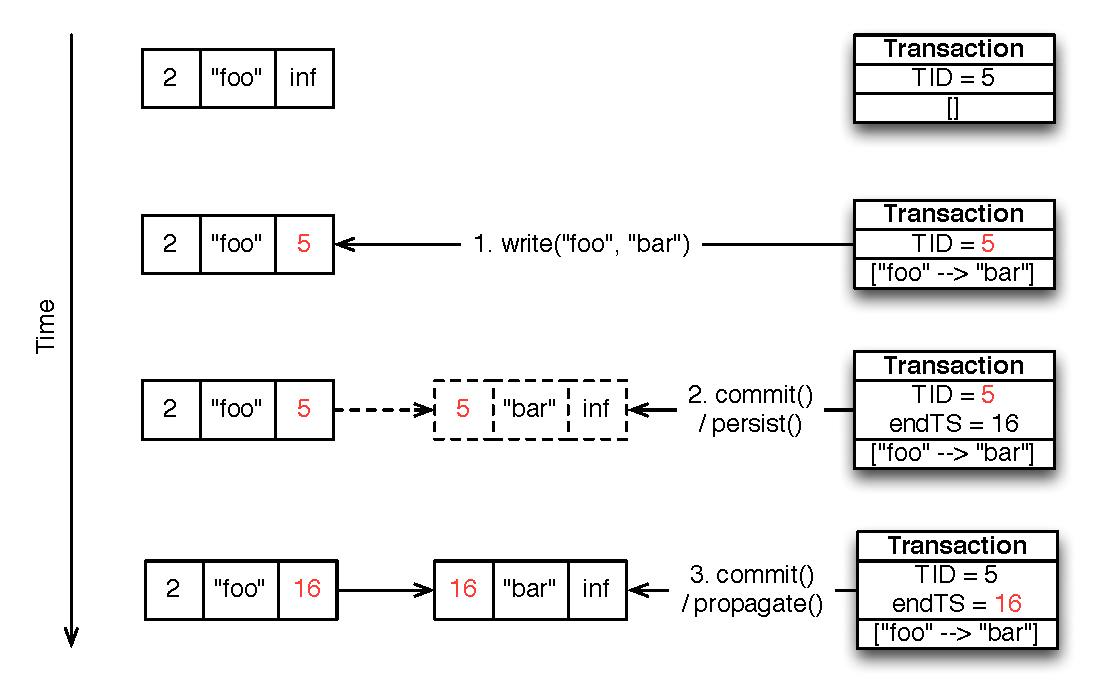
\includegraphics[scale=0.7]{figures/impl/mvcc.pdf}
%     \caption{Replacing the TID with end timestamp when committing an update.}
%     \label{fig:mvcc-updates}
% \end{figure}

